\section{Implementierung}
Dieses Kapitel beschreibt die Umsetzung des Projekts im Detail. Es wird ein Überblick über den Implementierungsprozesse gegeben, der Vorgehensweise bei der Entwicklung und ein Einblick in Probleme, welche während der Entwicklung aufgetreten sind.
Neben einer schrittweisen Darstellung der Implementierung werden auch exemplarisch Codebeispiele vorgestellt.
\subsection[Implementierungsdetails]{Implementierungsdetails}
In den Implementieungsdetails werden die Vorgehensweisen und Konzepte, welche für die Implementierung des Fontends und Backends benötigt werden, erläutert.

\subsubsection[Frontend]{Frontend}
Das \gls{sapui5}-Framework verwendet zur Darstellung der Seiten sogenannte \textit{Views} welche in \gls{xml} Dateien definiert werden.
Diese Views müssen mit der Dateiendung "\textbf{.view.xml}"\ enden, damit sie von \gls{sapui5} als View erkannt werden.

Views sind eine Art Kontainer für \gls{sapui5}-Elemente (Buttons, Input Felder, Tabellen, Listen, ...) und \gls{sapui5}-Layouts (Flex Box, HBox, VBox).
Views können jedoch auch andere Views beinhalten und so einen verschachtelten Aufbau der Seite schaffen.
Die \gls{sapui5}-Elemente sind vorgefertigte Komponenten welche von \gls{sapui5} bereitgestellt werden, um eine einheitliche Benutzeroberfläche zu schaffen, welche dann auch über verschiedene SAP-Anwendungen in einem Unternehmen konsistent ist.

Für die Admin-UI Seite sollen die Views und Komponenten wie in Abbildung \ref{fig:appstructure} angeortnent und strukturiert werden.
Die Unterseiten für die Eingabefelder aus den Anforderungen \ref{Tab:A4}, \ref{Tab:A5} und \ref{Tab:A6} werden in eigenen Views angezeigt, zwischen denen der Benutzer über die Navigationsleiste wechseln kann.

\begin{figure}[H]
    \centering
    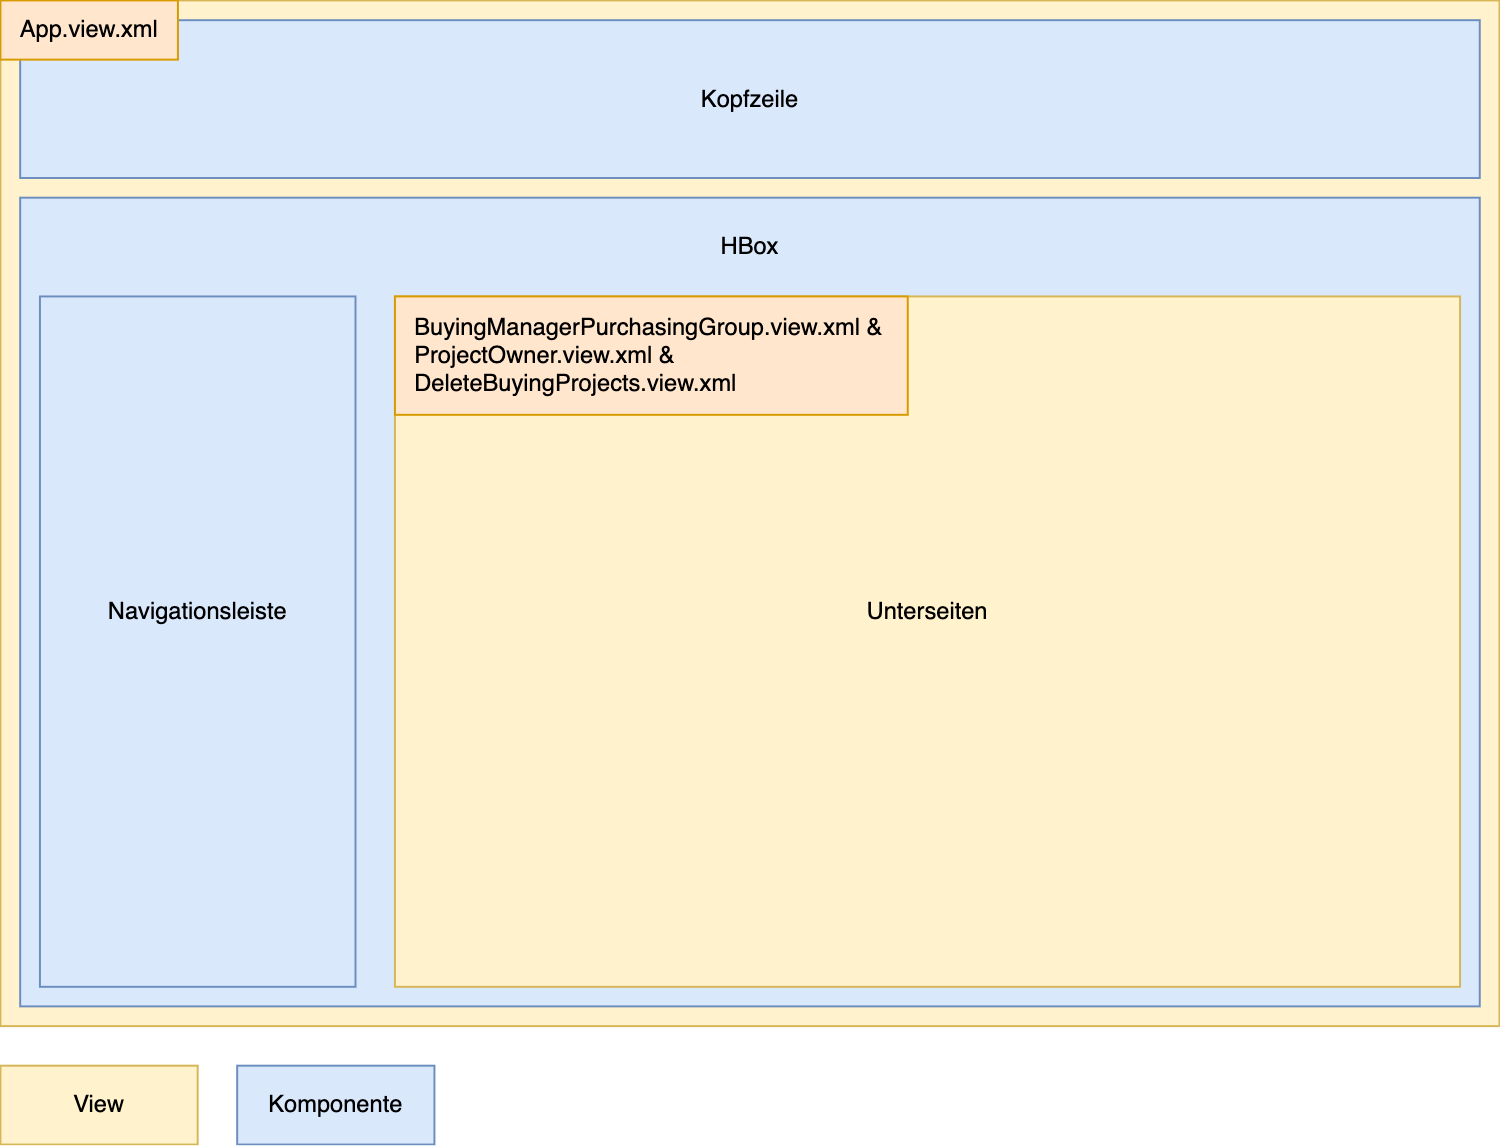
\includegraphics[width=\linewidth]{Images/AppStructure.png}
    \caption[Darstellung der Anwendungsstruktur]{Darstellung der Anwendungsstruktur}
    \label{fig:appstructure}
\end{figure}

Für jeden View kann ein \textit{Controller} erstellt werden, welcher die Funktionalität für die Views bereitstellt und Elemente dynamisch laden kann. 
Ein muss, so wie die View, eine besondere Dateiendung haben, damit \gls{sapui5} die Datei als Controller erkennen kann. Für Controller ist diese Endung "\textbf{.controller.ts}".

Für das Admin-UI soll für jeden View ein Controller erstellt werden. Zudem soll es einen sogenannten \textit{BaseContoller} geben, von dem alle anderen Controller seine Funktionen erben.
Dieser BaseController benötigt, anders also normale Controller, nicht die Controller spezifische Endung sondern nur die TypeScript spezifische Dateiendung "\textbf{.ts}".
Denn der BaseController wird keinem View explizit zugeordnet und muss daher auch nicht von \gls{sapui5} als Controller erkannt werden.  

Die Funktion eines BaseControllers ist es, Funktionen, welche von jedem Controller benötigt werden, in diesem zu definieren, damit diese an einer zentralen Stelle definiert sind und nicht in jedem Controller neu defniert werden müssen. 
Dazu gehören meist Helferfunktionen für zum Beispiel das Routing oder im Fall des Admin-UIs auch die Funktionalität der Aktionsleiste (siehe Anforderung \ref{Tab:A7}), welche auf jeder Unterseite eine sehr ähnliche Funktion hat.

In den Controllern für die einzelnen Unterseiten sollen Funktionen die spezifisch für die Unterseiten sind stehen, wie die intelligenten Vorschläge für die Eingabefelder (Anforderung \ref{Tab:A3}) und das Senden der Daten an das Backend.

\subsubsection[Backend]{Backend}
Im Backend sollen die Daten, welche von dem Frontend gesendet wurden, validiert und verarbeitet werden.

Für das Löschen einen Kaufprojekts muss jediglich die \textit{projectId} des zu löschenden Projektes gesendet werden, wofür eine \gls{cap} \textit{function} verwendet werden soll.
Eine \gls{cap} \textit{function} kann Parameter haben und muss immer einen Rückgabewert haben und führt eine gewisse Aktion aus.

Für das Ändern der Projekt Owner und Manager, sowie der Purchasing Organisation, soll für jede Änderung ein neuer Eintag in eine Datenbanktabelle geschrieben werden, der die alten und neuen Werte, sowie den Benutzer der die Änderung getätigt hat und den Zeitpunkt der Änderung beinhaltet.
Diese Datenbanktabellen sind in Abbildung \ref{fig:masschangetables} dargestellt.
Dies soll dazu dienen, die Änderungen auch im Nachhinein nachvollziehen zu können oder auch Rückgeängig zu machen. 

\begin{figure}[H]
    \centering
    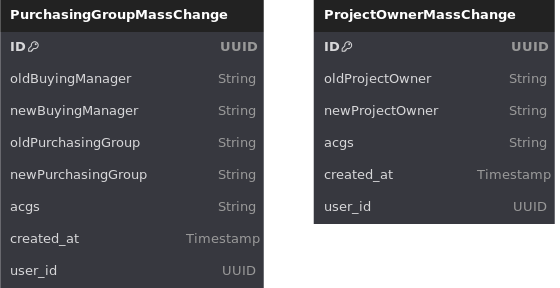
\includegraphics[width=.6\linewidth]{Images/MassChangeTables.png}
    \caption[Datenbanktabellen für Massenänderungen]{Datenbanktabellen für Massenänderungen}
    \label{fig:masschangetables}
\end{figure}

Wenn aus dem Frontend ein neuer Eintrag in einer der Tabelle erstellt wird, soll mit einer sogenannten \textit{Hook} in \gls{cap} das Änderen der Daten geschehen.
Diese \textit{Hooks} fangen das Erstellen der Tabelle ab und führen dann individuellen Code aus, in dem die gesendeten Daten verarbeitet werden können.

Bevor jedoch die Daten verarbeitet werden, muss überprüft werden, ob der Benutzer, der die Daten gesendet hat, die Berechtigung hat diese Änderungen durchzuführen.
Falls dies nicht der Fall ist, soll ein Error an das Frontend gesendet werden und eine entsprechende Errornachricht angezeigt werden.
Wenn der Benutzer jedoch die benötigte Berechtigung besitzt sollen die Daten verarbeitet und validiert werden und die Änderungen in der Datenbank vorgenommen werden.

\subsection[Schrittweise Beschreibung der Implementierung]{Schrittweise Beschreibung der Implementierung}

\subsection[Codebeispiele und Erklärungen]{Codebeispiele und Erklärungen}

\subsection[Herausforderungen und Problemlösungen]{Herausforderungen und Problemlösungen}

\subsection[Darstellung aufgetretener Herausforderungen]{Darstellung aufgetretener Herausforderungen}

\subsection[Beschreibung der Lösungsansätze]{Beschreibung der Lösungsansätze}
